\documentclass[12pt, letterpaper]{report}
\usepackage[margin=1in]{geometry}
\usepackage[utf8]{inputenc}
\usepackage{graphicx}
\usepackage{amsmath}
\usepackage{float}
\usepackage{subfig}
\graphicspath{ {./img/} }
\setlength\parindent{0pt}
\renewcommand{\thesection}{\Roman{section}.}
\renewcommand{\thesubsection}{\alph{subsection}.}


\title{CS1675 - Assignment 9}
\author{Zachary M. Mattis}


\begin{document}

\maketitle

\section{Problem 1 - K-Means Clustering}

S = \{(0,0)(0,5)(7,0)(6,7)\}

\[ d(\vec{p},\vec{q}) = \sqrt{\sum_{i=1}^{n} (q_i-p_i)^2} \]

% A
\subsection{Start: $\mu_1=(0,0), \mu_2=(7,0)$}

After Convergence w/ Euclidean Algorithm:
\\
\begin{table}[H]
	\centering
	\begin{tabular}{ l c l }
		$\mu_1=(0,2.5)$ & \qquad &  $\mu_2=(6.5,3.5)$ \\ \\
		$S_1 = \{(0,0),(0,5)\}$ & \qquad & $S_2 = \{(7,0),(6,7)\}$
	\end{tabular}
\end{table}

% B
\subsection{Start: $\mu_1=(3,3), \mu_2=(7,0)$}

After Convergence w/ Euclidean Algorithm:
\\
\begin{table}[H]
	\centering
	\begin{tabular}{ l c l }
		$\mu_1=(2,4)$ & \qquad &  $\mu_2=(7,0)$ \\ \\
		$S_1 = \{(0,0),(0,5),(6,7)\}$ & \qquad & $S_2 = \{(7,0)\}$
	\end{tabular}
\end{table}

\pagebreak
\section{Problem 2 - K-Means Clustering Experiments}

% A
\subsection{K = 3}

\begin{table}[H]
	\centering
	\begin{tabular}{ |r|r|r|r| }
		\hline
		& \textbf{$S_1$} & \textbf{$S_2$} & \textbf{$S_3$} \\
		\hline
		\textbf{$\mu$} & (3.94, 4.04) & (2.94, -4.97) & (0.86, 2.03) \\
		\hline
		\textbf{Total} & 66 & 36 & 98 \\
		\hline
		\textbf{Plot Color} & green & red & blue \\
		\hline
	\end{tabular}
	\caption{clustering\_data.txt}
\end{table}


\begin{figure}[H]
	\centering
	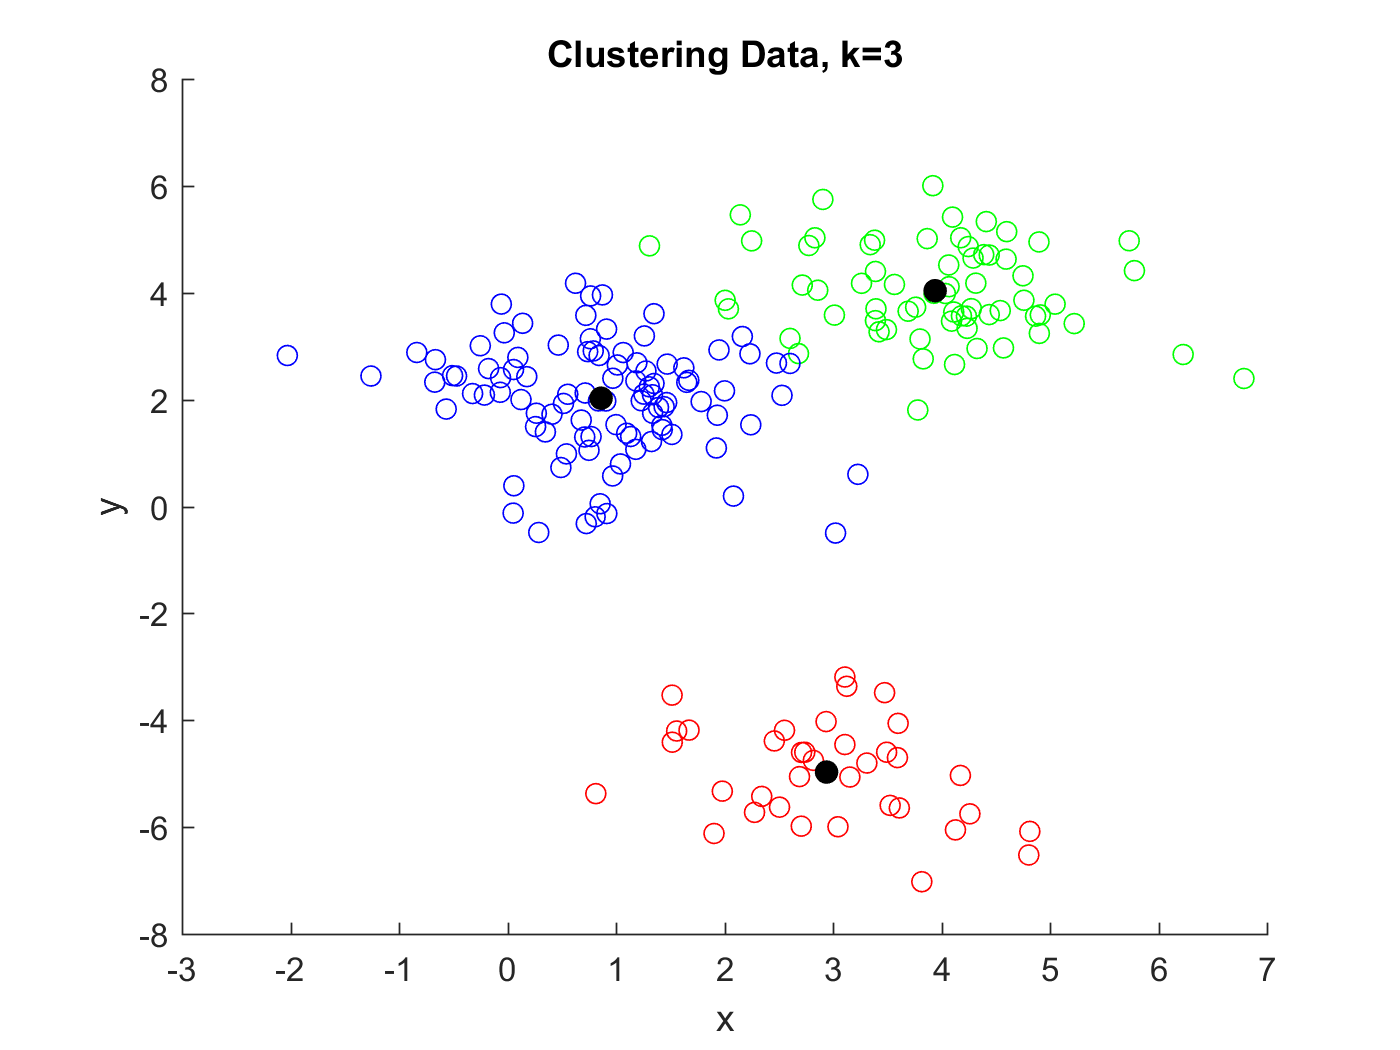
\includegraphics[width=0.7\columnwidth]{cluster_k3.png}
	\caption{clustering\_data.txt}
\end{figure}

\pagebreak
% B
\subsection{K = 4}

NOTE: Given the clustering of the data, running the algorithm on this dataset often yields different clusterings due to the starting points for the means. This concept is illustrated above from the differing resulting sets of Problem I, Parts A and B.
\\
\begin{table}[H]
	\centering
	\begin{tabular}{ |r|r|r|r|r| }
		\hline
		& \textbf{$S_1$} & \textbf{$S_2$} & \textbf{$S_3$} & \textbf{$S_4$} \\
		\hline
		\textbf{$\mu$} & (4.04, 4.03) & (0.68, 2.73) & (2.94, -4.97) & (1.23, 1.04) \\
		\hline
		\textbf{Total} & 63 & 61 & 36 & 40  \\
		\hline
		\textbf{Plot Color} & red & green & blue & cyan \\
		\hline
	\end{tabular}
	\caption{clustering\_data.txt}
\end{table}


\begin{figure}[H]
	\centering
	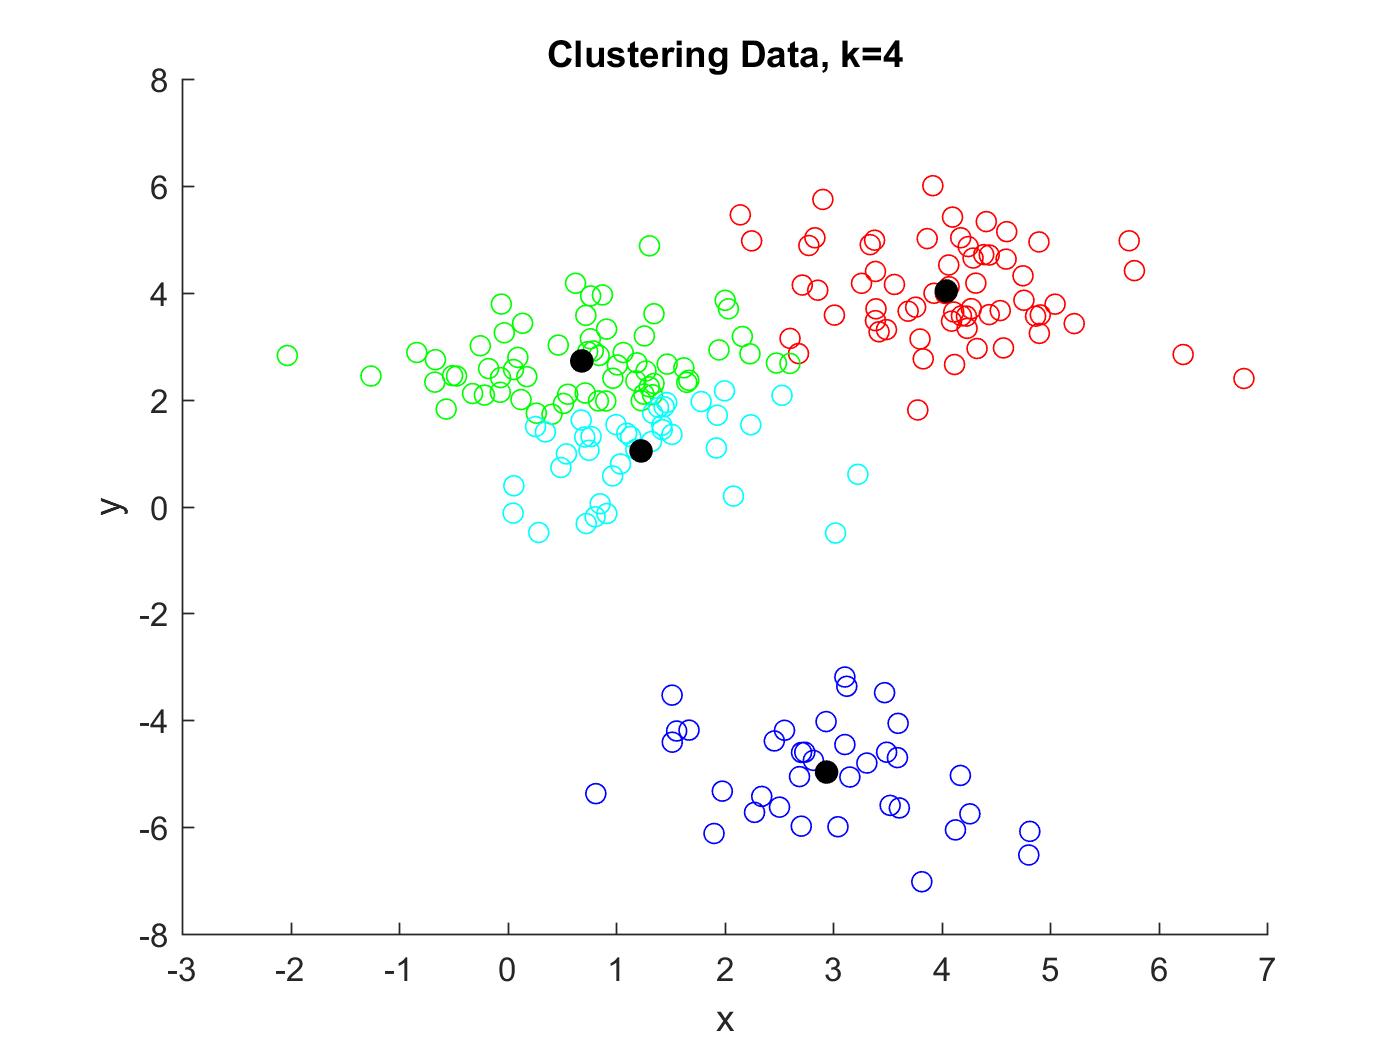
\includegraphics[width=0.7\columnwidth]{cluster_k4_alpha.png}
	\caption{clustering\_data.txt}
\end{figure}


% C
\subsection{Different Starting Means}


\begin{figure}[H]
	\centering
	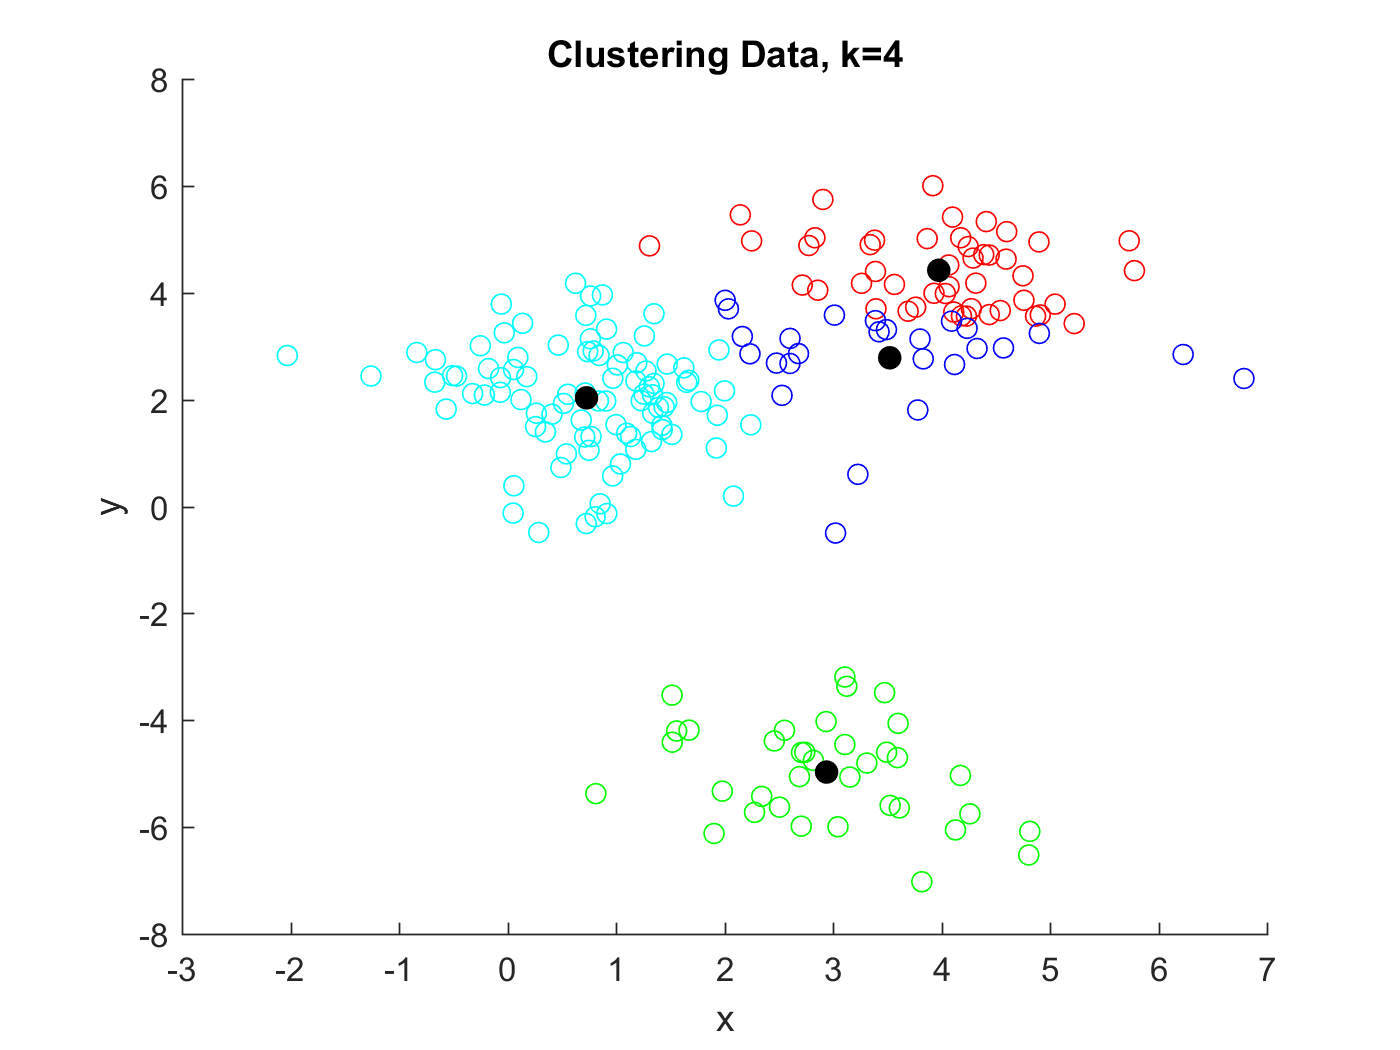
\includegraphics[width=0.7\columnwidth]{cluster_k4_delta.png}
	\caption{clustering\_data.txt}
\end{figure}

% D
\subsection{K-Means Optimizations}

Since the K-Means algorithm optimizes a distance metric, such as Euclidean Distance, it makes sense to compare the effectiveness of two different clustering via this measurement. For instance, the total distance between n data points for each given $k^{\text{th}}$ set is given by eq. \ref{eq:EuclideanDistance}. By summing individual distance for each set $S \in k$, the overall effectiveness of each algorithm instance can be compared, as seen in eq. \ref{eq:KMean}. Whichever algorithm instance produces the minimum total distance can be viewed as most effective.
\\ \\
\begin{equation}
\label{eq:EuclideanDistance}
d(\vec{x},\mu_k) = \sqrt{\sum_{i=1}^{n} (\mu_k-x_i)^2}
\end{equation}
\\
\begin{equation}
\label{eq:KMean}
\text{total distance}  = \sum_{j=1}^{k} d(\vec{x},\mu_k)
\end{equation}

% E
\subsection{Random K-Means Initialization}

\begin{table}[H]
	\centering
	\begin{tabular}{ |r|r|r|r| }
		\hline
		& \textbf{Run 1} & \textbf{Run 2} & \textbf{Run 3} \\
		\hline
		\textbf{Cluster Sizes} & 40,36,63,61 & 38,36,63,63 & 63,52,36,49 \\
		\hline
		\textbf{Total Distance} & 281.9109 & 281.9388 & 282.4565 \\
		\hline
	\end{tabular}
	\caption{Random Initialization Analysis}
\end{table}


\begin{figure}[H]
	\centering
	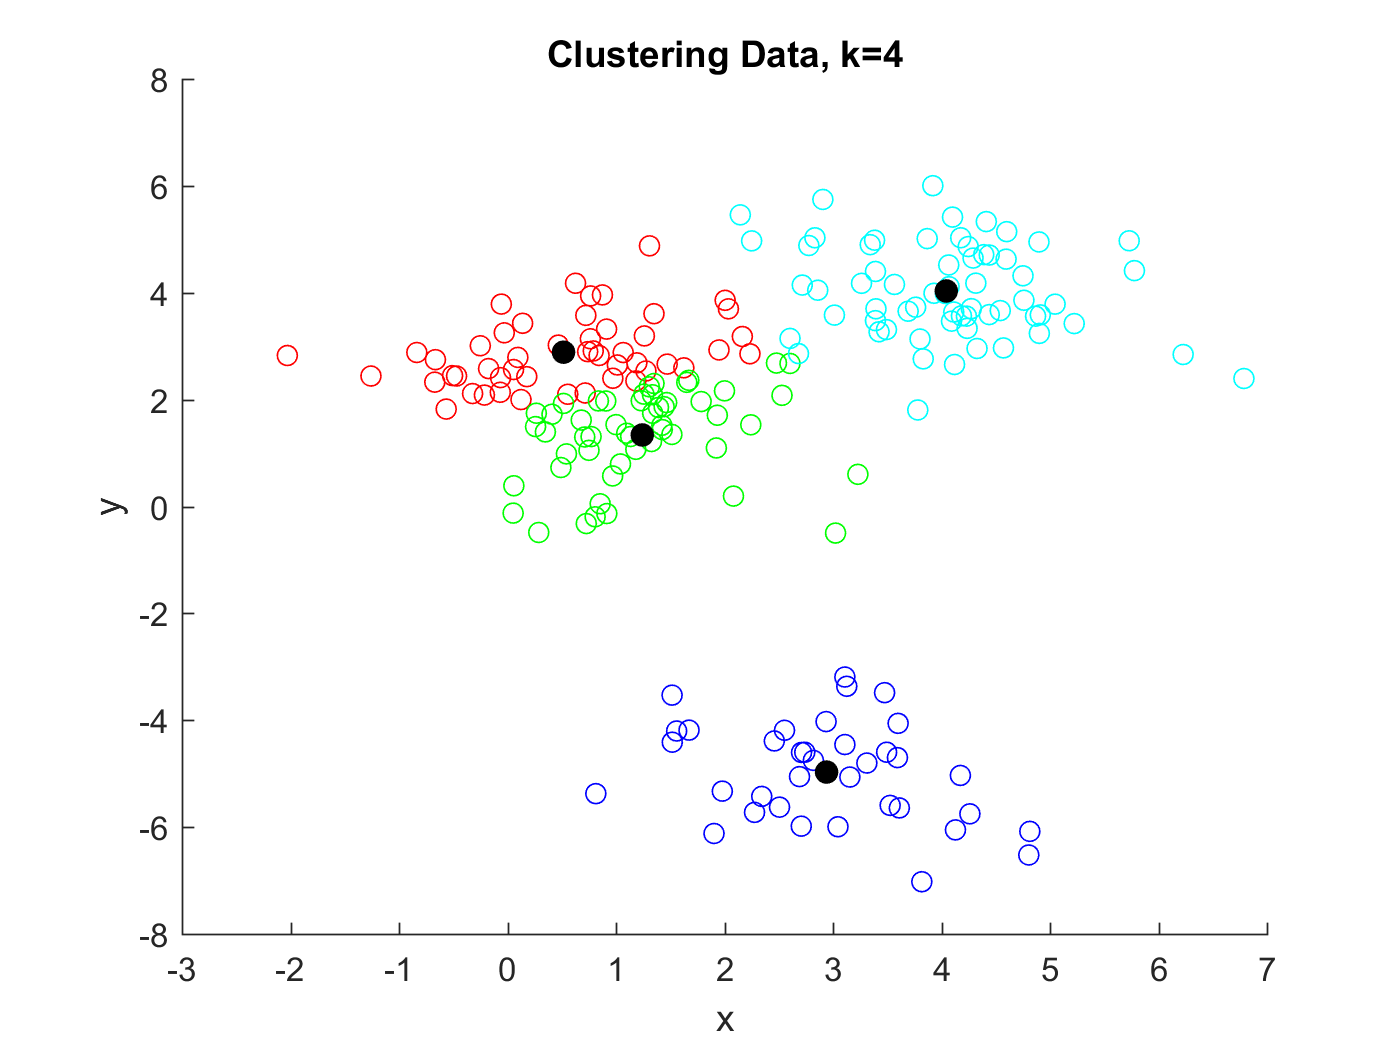
\includegraphics[width=0.7\columnwidth]{cluster_k4_opt.png}
	\caption{Optimal K=4}
\end{figure}

\section{Hierarchical Clustering}

% A
\subsection{Hierarchy of Clusters}

\begin{figure}[H]
	\centering
	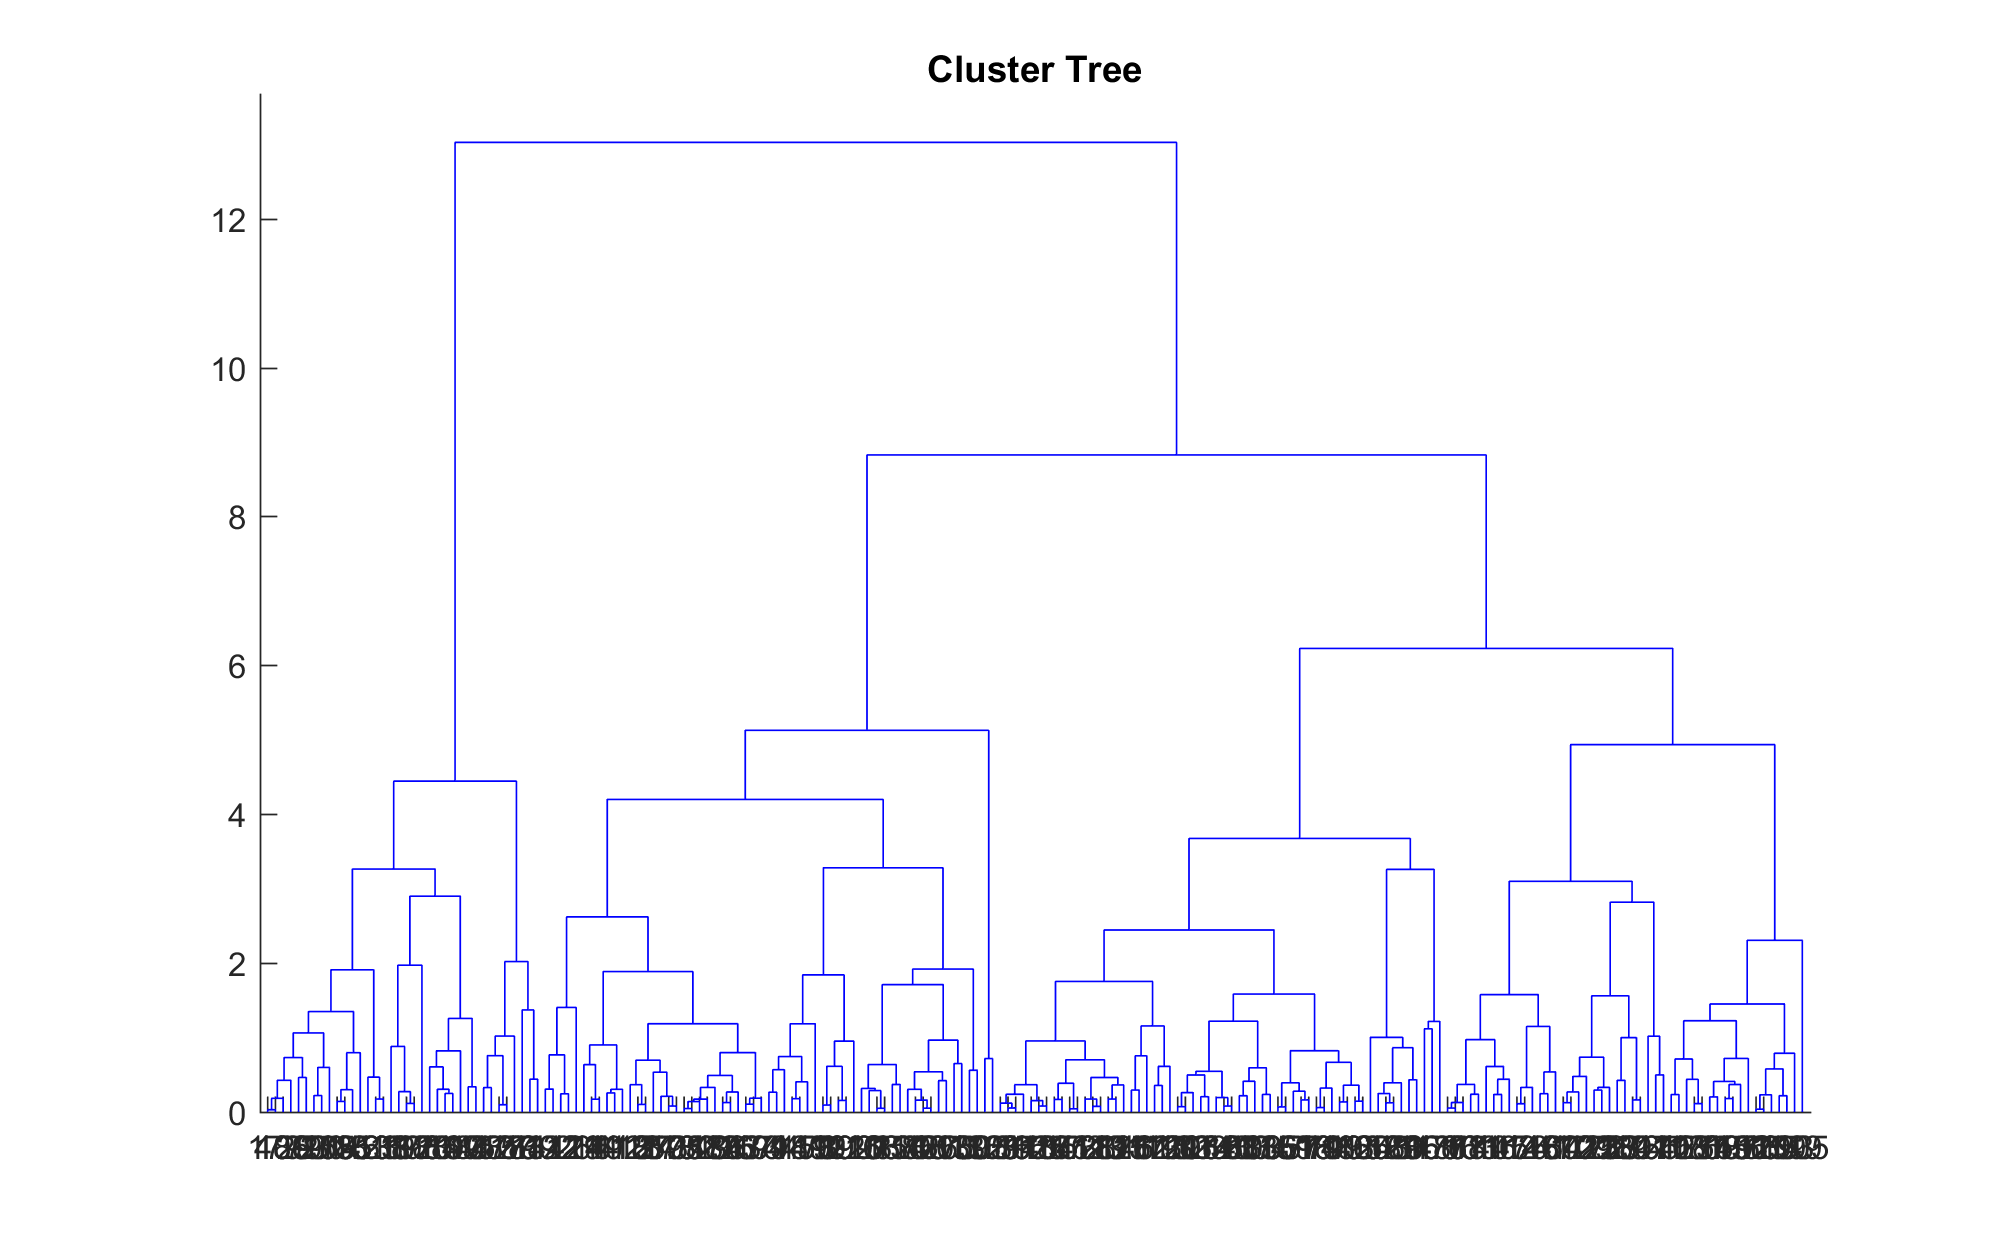
\includegraphics[width=0.6\columnwidth]{dendrogram.png}
	\caption{Dendrogram}
\end{figure}

% B
\subsection{Cluster Tree}

The clusters for both my K-Means algorithm implementation and the built-in Matlab \mbox{linkage()} and \mbox{cluster()} functions produced the same clustering of data. This makes sense, as each technique optimizes the a distance metric to produce the best result set.

\begin{figure}[H]
	\centering
	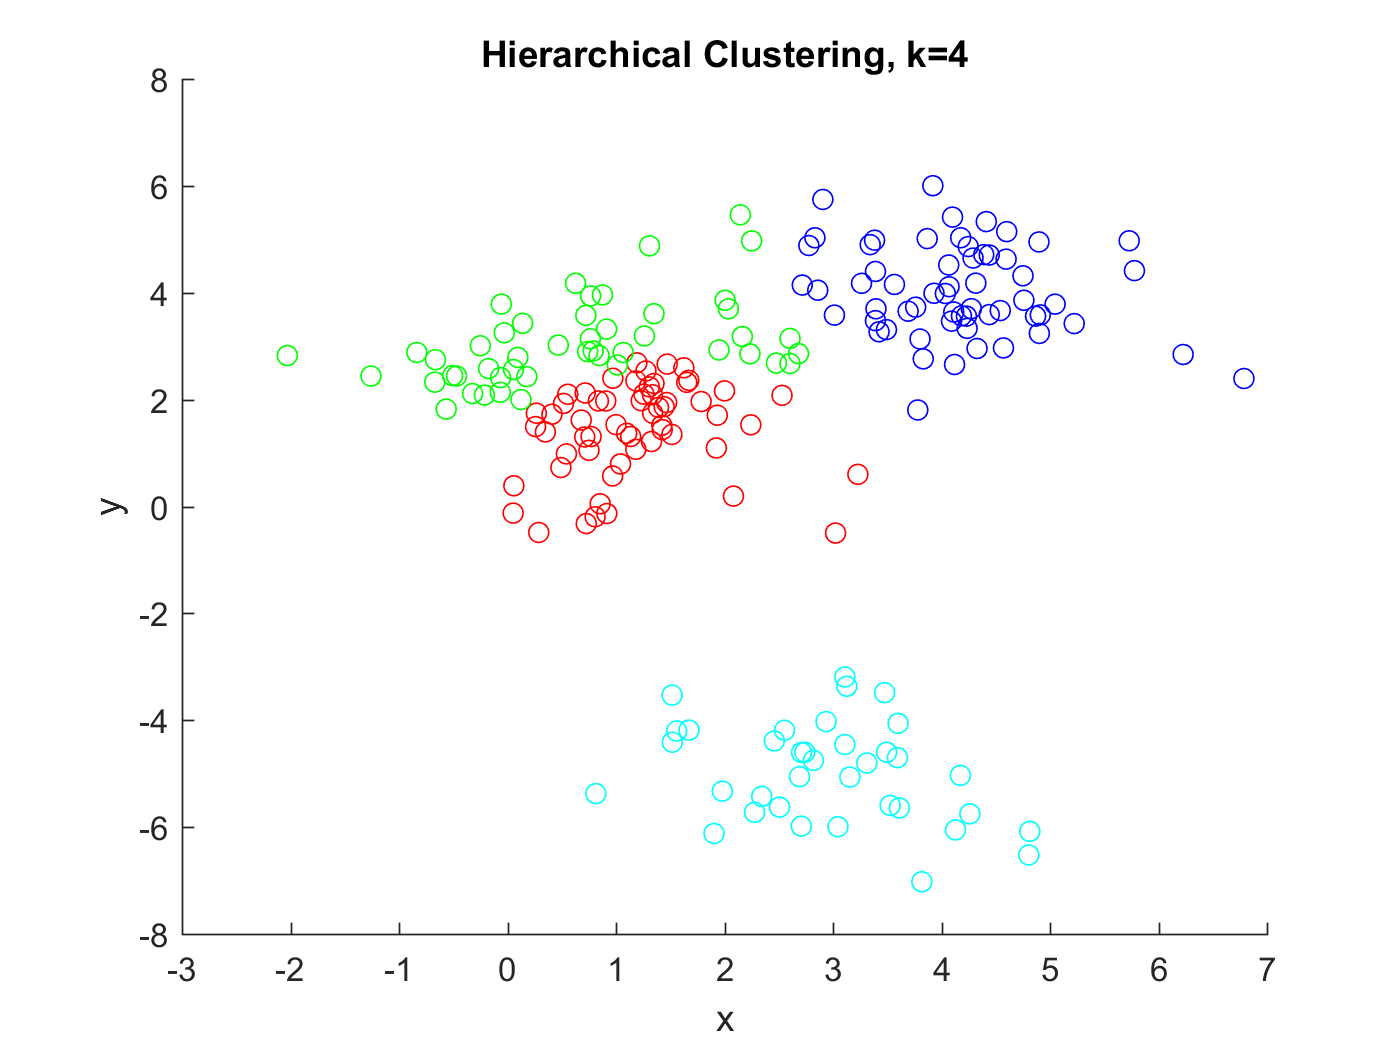
\includegraphics[width=0.7\columnwidth]{cluster_hierarchical.png}
	\caption{Cluster Tree}
\end{figure}


\end{document}